\documentclass[a4paper,11pt]{article}
\usepackage[T5]{fontenc}
\usepackage{lmodern,newunicodechar}
% Original mappings: Copyright 2005 Werner Lemberg <wl@gnu.org>.
% Adaptation for newunicodechar: LPPL version 1.3 or newer.
% Unicode to T5 mappings adapted from VNTeX t5enc.dfu (LPPL 1.3+).
\makeatletter
\newunicodechar{«}{\guillemotleft}
\newunicodechar{»}{\guillemotright}
\newunicodechar{À}{\@tabacckludge`A}
\newunicodechar{Á}{\@tabacckludge'A}
\newunicodechar{Â}{\^A}
\newunicodechar{Ã}{\~A}
\newunicodechar{È}{\@tabacckludge`E}
\newunicodechar{É}{\@tabacckludge'E}
\newunicodechar{Ê}{\^E}
\newunicodechar{Ì}{\@tabacckludge`I}
\newunicodechar{Í}{\@tabacckludge'I}
\newunicodechar{Ò}{\@tabacckludge`O}
\newunicodechar{Ó}{\@tabacckludge'O}
\newunicodechar{Ô}{\^O}
\newunicodechar{Õ}{\~O}
\newunicodechar{Ù}{\@tabacckludge`U}
\newunicodechar{Ú}{\@tabacckludge'U}
\newunicodechar{Ý}{\@tabacckludge'Y}
\newunicodechar{à}{\@tabacckludge`a}
\newunicodechar{á}{\@tabacckludge'a}
\newunicodechar{â}{\^a}
\newunicodechar{ã}{\~a}
\newunicodechar{è}{\@tabacckludge`e}
\newunicodechar{é}{\@tabacckludge'e}
\newunicodechar{ê}{\^e}
\newunicodechar{ì}{\@tabacckludge`\i}
\newunicodechar{í}{\@tabacckludge'\i}
\newunicodechar{ò}{\@tabacckludge`o}
\newunicodechar{ó}{\@tabacckludge'o}
\newunicodechar{ô}{\^o}
\newunicodechar{õ}{\~o}
\newunicodechar{ù}{\@tabacckludge`u}
\newunicodechar{ú}{\@tabacckludge'u}
\newunicodechar{ý}{\@tabacckludge'y}
\newunicodechar{Ă}{\u A}
\newunicodechar{ă}{\u a}
\newunicodechar{Đ}{\DJ}
\newunicodechar{đ}{\dj}
\newunicodechar{Ĩ}{\~I}
\newunicodechar{ĩ}{\~\i}
\newunicodechar{ı}{\i}
\newunicodechar{Ũ}{\~U}
\newunicodechar{ũ}{\~u}
\newunicodechar{Ơ}{\OHORN}
\newunicodechar{ơ}{\ohorn}
\newunicodechar{Ư}{\UHORN}
\newunicodechar{ư}{\uhorn}
\newunicodechar{Ạ}{\d A}
\newunicodechar{ạ}{\d a}
\newunicodechar{Ả}{\h A}
\newunicodechar{ả}{\h a}
\newunicodechar{Ấ}{\@tabacckludge'\ACIRCUMFLEX}
\newunicodechar{ấ}{\@tabacckludge'\acircumflex}
\newunicodechar{Ầ}{\@tabacckludge`\ACIRCUMFLEX}
\newunicodechar{ầ}{\@tabacckludge`\acircumflex}
\newunicodechar{Ẩ}{\h\ACIRCUMFLEX}
\newunicodechar{ẩ}{\h\acircumflex}
\newunicodechar{Ẫ}{\~\ACIRCUMFLEX}
\newunicodechar{ẫ}{\~\acircumflex}
\newunicodechar{Ậ}{\d\ACIRCUMFLEX}
\newunicodechar{ậ}{\d\acircumflex}
\newunicodechar{Ắ}{\@tabacckludge'\ABREVE}
\newunicodechar{ắ}{\@tabacckludge'\abreve}
\newunicodechar{Ằ}{\@tabacckludge`\ABREVE}
\newunicodechar{ằ}{\@tabacckludge`\abreve}
\newunicodechar{Ẳ}{\h\ABREVE}
\newunicodechar{ẳ}{\h\abreve}
\newunicodechar{Ẵ}{\~\ABREVE}
\newunicodechar{ẵ}{\~\abreve}
\newunicodechar{Ặ}{\d\ABREVE}
\newunicodechar{ặ}{\d\abreve}
\newunicodechar{Ẹ}{\d E}
\newunicodechar{ẹ}{\d e}
\newunicodechar{Ẻ}{\h E}
\newunicodechar{ẻ}{\h e}
\newunicodechar{Ẽ}{\~ E}
\newunicodechar{ẽ}{\~ e}
\newunicodechar{Ế}{\@tabacckludge'\ECIRCUMFLEX}
\newunicodechar{ế}{\@tabacckludge'\ecircumflex}
\newunicodechar{Ề}{\@tabacckludge`\ECIRCUMFLEX}
\newunicodechar{ề}{\@tabacckludge`\ecircumflex}
\newunicodechar{Ể}{\h\ECIRCUMFLEX}
\newunicodechar{ể}{\h\ecircumflex}
\newunicodechar{Ễ}{\~\ECIRCUMFLEX}
\newunicodechar{ễ}{\~\ecircumflex}
\newunicodechar{Ệ}{\d\ECIRCUMFLEX}
\newunicodechar{ệ}{\d\ecircumflex}
\newunicodechar{Ỉ}{\h I}
\newunicodechar{ỉ}{\h i}
\newunicodechar{Ị}{\d I}
\newunicodechar{ị}{\d i}
\newunicodechar{Ọ}{\d O}
\newunicodechar{ọ}{\d o}
\newunicodechar{Ỏ}{\h O}
\newunicodechar{ỏ}{\h o}
\newunicodechar{Ố}{\@tabacckludge'\OCIRCUMFLEX}
\newunicodechar{ố}{\@tabacckludge'\ocircumflex}
\newunicodechar{Ồ}{\@tabacckludge`\OCIRCUMFLEX}
\newunicodechar{ồ}{\@tabacckludge`\ocircumflex}
\newunicodechar{Ổ}{\h\OCIRCUMFLEX}
\newunicodechar{ổ}{\h\ocircumflex}
\newunicodechar{Ỗ}{\~\OCIRCUMFLEX}
\newunicodechar{ỗ}{\~\ocircumflex}
\newunicodechar{Ộ}{\d\OCIRCUMFLEX}
\newunicodechar{ộ}{\d\ocircumflex}
\newunicodechar{Ớ}{\@tabacckludge'\OHORN}
\newunicodechar{ớ}{\@tabacckludge'\ohorn}
\newunicodechar{Ờ}{\@tabacckludge`\OHORN}
\newunicodechar{ờ}{\@tabacckludge`\ohorn}
\newunicodechar{Ở}{\h\OHORN}
\newunicodechar{ở}{\h\ohorn}
\newunicodechar{Ỡ}{\~\OHORN}
\newunicodechar{ỡ}{\~\ohorn}
\newunicodechar{Ợ}{\d\OHORN}
\newunicodechar{ợ}{\d\ohorn}
\newunicodechar{Ụ}{\d U}
\newunicodechar{ụ}{\d u}
\newunicodechar{Ủ}{\h U}
\newunicodechar{ủ}{\h u}
\newunicodechar{Ứ}{\@tabacckludge'\UHORN}
\newunicodechar{ứ}{\@tabacckludge'\uhorn}
\newunicodechar{Ừ}{\@tabacckludge`\UHORN}
\newunicodechar{ừ}{\@tabacckludge`\uhorn}
\newunicodechar{Ử}{\h\UHORN}
\newunicodechar{ử}{\h\uhorn}
\newunicodechar{Ữ}{\~\UHORN}
\newunicodechar{ữ}{\~\uhorn}
\newunicodechar{Ự}{\d\UHORN}
\newunicodechar{ự}{\d\uhorn}
\newunicodechar{Ỳ}{\@tabacckludge`Y}
\newunicodechar{ỳ}{\@tabacckludge`y}
\newunicodechar{Ỵ}{\d Y}
\newunicodechar{ỵ}{\d y}
\newunicodechar{Ỷ}{\h Y}
\newunicodechar{ỷ}{\h y}
\newunicodechar{Ỹ}{\~Y}
\newunicodechar{ỹ}{\~y}
\newunicodechar{‌}{\textcompwordmark}
\newunicodechar{–}{\textendash}
\newunicodechar{—}{\textemdash}
\newunicodechar{‘}{\textquoteleft}
\newunicodechar{’}{\textquoteright}
\newunicodechar{‚}{\quotesinglbase}
\newunicodechar{“}{\textquotedblleft}
\newunicodechar{”}{\textquotedblright}
\newunicodechar{„}{\quotedblbase}
\newunicodechar{‰}{\textperthousand}
\newunicodechar{‱}{\textpertenthousand}
\newunicodechar{‹}{\guilsinglleft}
\newunicodechar{›}{\guilsinglright}
\newunicodechar{␣}{\textvisiblespace}
\newunicodechar{–}{\textendash}
\newunicodechar{—}{\textemdash}
\newunicodechar{×}{\ensuremath{\times}}
\newunicodechar{“}{\textquotedblleft}
\newunicodechar{”}{\textquotedblright}
\makeatother

\usepackage[left=2cm,right=2cm,top=2cm,bottom=2cm]{geometry}
\usepackage{amsmath,amssymb,graphicx,booktabs,array,float,caption,fvextra,titlesec,tocloft,needspace}
\usepackage[unicode,hidelinks]{hyperref}
\hypersetup{pdftitle={Báo cáo HRI -- Bài thực hành 06: Điều khiển TurtleBot 4 bằng cử chỉ tay},pdfauthor={Đỗ Việt Anh}}
\setlength{\parindent}{0pt}
\setlength{\parskip}{5pt}
\setlength{\emergencystretch}{3em}
\setlength{\tabcolsep}{4pt}
\renewcommand{\arraystretch}{1.14}
\renewcommand{\contentsname}{Mục lục}
\renewcommand{\figurename}{Hình}
\renewcommand{\tablename}{Bảng}
\titleformat{\section}{\large\bfseries}{\thesection}{.7em}{}[\titlerule]
\titlespacing*{\section}{0pt}{13pt}{8pt}
\titleformat{\subsection}{\normalsize\bfseries}{\thesubsection}{.7em}{}
\titlespacing*{\subsection}{0pt}{9pt}{5pt}
\captionsetup{font={small,it},labelfont={bf,up},labelsep=colon,skip=5pt}
\setlength{\cftbeforesecskip}{3pt}
\setcounter{tocdepth}{1}
\fvset{fontsize=\small,breaklines=true,breakanywhere=true,breaksymbolleft={},frame=single,framesep=4pt}
\newcommand{\code}[1]{\nolinkurl{#1}}
\newcommand{\fig}[3]{\begin{figure}[H]\centering\includegraphics[width=#2\linewidth]{#1}\caption{#3}\end{figure}}
\newcommand{\github}{https://github.com/vanhhhhh512/turtlebot4_bai06}
\newcommand{\drive}{https://drive.google.com/drive/folders/1FdF8vADL3xgHH5QPhekMk_7wn1XFR4Jp?usp=drive_link}
\raggedbottom
\begin{document}
\hypersetup{pageanchor=false}
\begin{titlepage}
\thispagestyle{empty}\centering
\vspace*{1.5cm}
{\large\bfseries ĐẠI HỌC QUỐC GIA HÀ NỘI\\[3pt]TRƯỜNG ĐẠI HỌC CÔNG NGHỆ\par}
\vspace{.5cm}

\includegraphics[width=3.2cm]{uet_logo.png}\par
\vspace{.35cm}
{\LARGE\bfseries BÁO CÁO HRI\par}
{\Large BÀI THỰC HÀNH 06\par}
\vspace{.2cm}
{\Large\bfseries GIAO TIẾP PHI NGÔN NGỮ\\[5pt]ĐIỀU KHIỂN TURTLEBOT 4\\[5pt]BẰNG CỬ CHỈ TAY\par}
\vspace{1.5cm}
\begin{tabular}{@{}ll@{}}
\textbf{Họ và tên sinh viên:}&Đỗ Việt Anh\\[8pt]
\textbf{Mã sinh viên:}&23020719\\[8pt]
\textbf{Lớp:}&K68E-RE\\[8pt]
\textbf{Giảng viên hướng dẫn:}&Kỹ sư Nguyễn Quốc Bảo
\end{tabular}
\vfill
Mã nguồn GitHub: \href{\github}{turtlebot4\_bai06}\\[4pt]
Video demo: \href{\drive}{Google Drive -- Bài 06}
\vspace{.3cm}
\end{titlepage}
\hypersetup{pageanchor=true}
\pagenumbering{arabic}
\tableofcontents
\section{Mục tiêu và môi trường sử dụng}
Bài thực hành sử dụng webcam laptop để nhận diện cử chỉ tay bằng OpenCV và
MediaPipe, sau đó điều khiển TurtleBot 4 trong Gazebo qua ROS 2. Người điều khiển
chọn hành vi bằng tay, xác nhận bằng ngón cái và có thể dừng hoặc hủy khi cần.
Các chuyển động trong phần demo được điều khiển bằng cử chỉ.

\begin{table}[H]\centering\small
\begin{tabular}{@{}p{3.6cm}p{12.4cm}@{}}\toprule
Thành phần & Môi trường sử dụng\\\midrule
Hệ điều hành, ROS & Ubuntu 22.04, ROS 2 Humble, Python 3.10.12.\\
Mô phỏng & TurtleBot 4 Standard, Ignition Gazebo Fortress.\\
Nhận diện & MediaPipe Gesture Recognizer 0.10.21, model \code{gesture_recognizer.task}.\\
Ảnh và hiển thị & OpenCV 4.11.0, NumPy 1.26.4, webcam laptop \code{/dev/video0}.\\
World & Sàn trống 12 × 12 m; giới hạn điều khiển \( |x|, |y| \leq 4{,}5\,\mathrm{m}\).\\\bottomrule
\end{tabular}
\caption{Môi trường triển khai Bài 06.}
\end{table}
\code{simulation_ready_node} kiểm tra và kích hoạt controller bánh xe rồi gọi
undock. Webcam luôn nhận diện tay; dòng trạng thái robot cho biết nếu chưa
ra khỏi dock hoặc thiếu odom. File cấu hình mô phỏng đặt chế độ lùi ngay khi
khởi động; node chuẩn bị đọc lại cấu hình trước khi cho điều khiển. Không có
bước xin quyền lùi bằng cử chỉ hoặc gửi cấu hình sau khi chọn hành vi.
\clearpage

\section{Cấu trúc hệ thống và luồng dữ liệu}
\fig{figures/system_flow.pdf}{1.0}{Hai node nhận diện và hành vi trao đổi qua topic ROS 2.}
\code{gesture_recognition_node} dùng OpenCV đọc ảnh, đổi BGR sang RGB và chạy
MediaPipe. Node lấy nhãn cùng điểm nhận diện, vẽ 21 điểm và đường nối bàn tay,
hiển thị trạng thái robot rồi publish kết quả mới qua \code{/detected_gesture}.

\code{robot_behavior_node} subscribe nhãn cử chỉ, lưu lựa chọn và chỉ phát vận tốc
sau xác nhận. Timer điều khiển chạy 20 Hz, độc lập với suy luận ảnh để tiếp tục
kiểm tra điều kiện dừng khi camera hoặc nhận diện bị gián đoạn.

\begin{table}[H]\centering\small
\begin{tabular}{@{}p{4.1cm}p{4.5cm}p{7.2cm}@{}}\toprule
Topic & Kiểu message & Vai trò\\\midrule
\code{/detected_gesture} & \code{std_msgs/msg/String} & Nhãn cử chỉ mới, kể cả \code{NO_HAND}/\code{UNKNOWN}.\\
\code{/cmd_vel} & \code{geometry_msgs/msg/Twist} & Vận tốc thẳng \code{linear.x} và quay \code{angular.z}.\\
\code{/odom} & \code{nav_msgs/msg/Odometry} & Quãng đường và góc quay thực hiện.\\
\code{/dock_status} & \code{irobot_create_msgs/msg/DockStatus} & Chặn chạy khi robot chưa ra khỏi dock.\\
\code{/hazard_detection} & \code{irobot_create_msgs/msg/HazardDetectionVector} & Nhận bump, cliff, stall, wheel drop.\\
\code{/behavior_status} & \code{std_msgs/msg/String} & JSON trạng thái, hành vi, pha và chu kỳ.\\\bottomrule
\end{tabular}
\caption{Các topic chính.}
\end{table}

\textbf{Các file trong package.}
\code{gesture_recognition_node.py} xử lý webcam và model;
\code{wave_detector.py} nhận chuyển động vẫy tay;
\code{visualization.py} vẽ khung tay.
\code{robot_behavior_node.py} quản lý hành vi và điều kiện dừng.
\code{config/gestures.yaml} lưu ngưỡng nhận diện, tốc độ và thời gian chờ.
\code{launch/demo.launch.py} mở Gazebo, bridge, robot và hai node;
\code{worlds/gesture_arena.sdf} tạo môi trường trống.
\clearpage

\section{Nhận diện và quy ước sáu cử chỉ}
\begin{table}[H]\centering\small
\begin{tabular}{@{}p{3.1cm}p{5.0cm}p{7.7cm}@{}}\toprule
Cử chỉ & Cách thực hiện & Hành vi\\\midrule
Wave & Xòe năm ngón rồi vẫy nhẹ các ngón hai lần. & Chọn chào: xoay trái, phải rồi về hướng gần ban đầu.\\
Pointing Up & Duỗi ngón trỏ lên, gập các ngón còn lại. & Chọn tiến--lùi 4 chu kỳ, tổng 8 chặng.\\
Victory & Duỗi ngón trỏ và ngón giữa thành chữ V. & Chọn đi theo quỹ đạo tròn một vòng.\\
Thumbs Up & Nắm các ngón và giơ ngón cái. & Xác nhận chạy hoặc tiếp tục tác vụ đang PAUSED.\\
Open Palm & Xòe cả năm ngón về phía camera. & Tạm dừng ngay, giữ hành vi và tiến độ.\\
Closed Fist & Nắm kín bàn tay. & Hủy hành vi và tiến độ, trở về trạng thái chờ.\\\bottomrule
\end{tabular}
\caption{Quy ước cử chỉ và hành vi. Mọi hành vi chuyển động đều cần xác nhận.}
\end{table}

\fig{figures/gesture_poses.pdf}{.94}{Sơ đồ minh họa sáu cử chỉ; Wave có chuyển động các ngón.}
\clearpage
\subsection{Landmarks và chuyển động các ngón}
\begin{minipage}[t]{.29\linewidth}\centering
\vspace{0pt}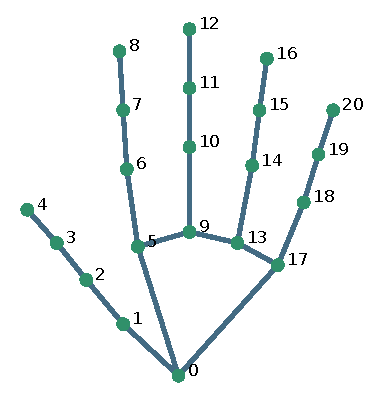
\includegraphics[width=.94\linewidth]{figures/hand_landmarks.pdf}
\captionof{figure}{Sơ đồ 21 điểm bàn tay.}
\end{minipage}\hfill
\begin{minipage}[t]{.67\linewidth}\vspace{0pt}
\textbf{Năm cử chỉ tĩnh.} MediaPipe trả về nhãn và confidence. Chương trình dùng
ngưỡng chung 0,60. Thumb Up nhận từ 0,55, duy trì từ 0,45 khi ngón cái duỗi và
các ngón còn lại co; mỗi frame vẫn cần model dự đoán \code{Thumb_Up} mới.
Confidence là điểm do model trả về, không phải độ chính xác của toàn hệ thống.

\textbf{Cử chỉ Wave.} Xòe năm ngón rồi vẫy nhẹ ít nhất ba ngón hai lần trong
4 s. Chương trình đo đầu ngón trong hệ tọa độ gắn với lòng bàn tay, lọc trung vị
ba mẫu và đếm từng ngón riêng. Các ngón có thể lắc hoặc co--duỗi lệch nhịp.
Tay mở đứng yên vẫn là Open Palm. Wave là luật theo landmarks, không phải class
có sẵn của model.
\end{minipage}

\textbf{Phân biệt Wave và Open Palm.}
Khi robot đang chạy, Open Palm được chuyển thẳng thành lệnh tạm dừng; không chờ nhận
Wave. Khi đang IDLE, Wave chỉ tạo lựa chọn chào. Cửa sổ hiển thị bộ đếm 3 s để
đổi từ tay mở sang Thumb Up; tay mở trong đoạn này giữ lựa chọn, không tạo lệnh
chạy. Hết đoạn chuyển mà vẫn mở tay thì chuyển PAUSED, giữ lựa chọn. UNKNOWN ngắn tối đa 0,18 s
không xóa các mẫu xác nhận; nó không xác nhận hành vi. Khi đang thu Wave, nắm
giữ 0,4 s mới hủy để phân biệt với pha co ngón; khi đang chạy, nắm tay hủy ngay.
Khi đang SELECTED, mất tay hủy lựa chọn.

Cửa sổ webcam hiển thị ảnh gương, khung tay, nhãn, điểm model và trạng thái robot.
Chỉ một tay được dùng để điều khiển. Kết quả có nhiều tay được coi là mơ hồ và làm
robot dừng. Sau xác nhận có thể bỏ tay khỏi ảnh; robot tự chạy hết tác vụ theo odom.
\fig{figures/wave_features.pdf}{.97}{Đặc trưng đầu ngón từ webcam thật. Vạch đỏ đánh dấu Wave; bộ đếm về 0 sau khi phát sự kiện.}
\clearpage

\section{Mô phỏng và chuẩn bị robot}
World có sàn trống 12 × 12 m, một TurtleBot 4 Standard và dock. Node chuẩn bị
kiểm tra controller bánh xe, cấu hình lùi và thực hiện undock. Hành vi chỉ được
xác nhận khi robot đã ra khỏi dock, có odometry mới và không có hazard.
\fig{figures/gazebo_arena.png}{.98}{Môi trường gesture\_arena trong Gazebo; robot và dock nằm trong vùng chạy trống.}
\fig{figures/gazebo_closeup.png}{.88}{TurtleBot 4 Standard và dock trong cùng phiên mô phỏng.}
\clearpage

\section{Điều khiển hành vi và cơ chế dừng}
\fig{figures/state_machine.pdf}{1.0}{Luồng chọn, xác nhận và thực hiện hành vi.}
\textbf{Chào.} Sau Wave rồi Thumb Up, robot quay trái khoảng 0,45 rad, quay phải
0,90 rad, sau đó quay trái 0,45 rad để trở về gần hướng ban đầu. Mỗi pha kết thúc
theo góc quay tích lũy từ odometry.

\textbf{Tiến--lùi.} Sau Pointing Up rồi Thumb Up, robot tiến 0,40 m và lùi 0,40 m
cho mỗi chu kỳ, lặp bốn chu kỳ. Tiến độ được tính bằng độ dời odom chiếu lên hướng
bắt đầu chặng. Giao diện hiển thị số chu kỳ từ 1/4 đến 4/4.
Trong Gazebo, launch cấu hình Create 3 ở chế độ \code{safety_override=backup_only}
để cho phép lùi hết 0,40 m; node vẫn kiểm tra hazard, vùng chạy và lệnh dừng.

\textbf{Đi tròn.} Sau Victory rồi Thumb Up, robot xoay tại chỗ để tâm vòng nằm xa
dock, rồi chạy với \(v=0{,}12\,\mathrm{m/s}\), \(\omega=0{,}20\,\mathrm{rad/s}\).
Bán kính cấu hình là \(R=v/\omega=0{,}60\,\mathrm{m}\). Robot dừng khi tổng góc quay
ở pha đi tròn đạt \(2\pi\), không chỉ dựa vào thời gian ước lượng.

\begin{table}[H]\centering\small
\begin{tabular}{@{}p{4.5cm}p{11.4cm}@{}}\toprule
Điều kiện & Xử lý trong chương trình\\\midrule
Cử chỉ chọn/xác nhận & Cần ít nhất 3 kết quả cùng nhãn, ổn định tối thiểu 0,2 s.\\
Giữ nguyên cử chỉ & Chỉ tạo một sự kiện; không chạy lại hoặc xếp thêm lệnh trong khi đang chạy.\\
Open Palm / Thumb Up & Phát Twist bằng 0 ngay, chuyển PAUSED và giữ tiến độ; Thumb Up xác nhận để tiếp tục.\\
Closed Fist & Hủy cả lựa chọn lẫn tiến độ, phát 0 và trở về IDLE.\\
NO\_HAND / UNKNOWN mới & Sau xác nhận, tác vụ tiếp tục theo odom; ở SELECTED, bỏ tay hủy lựa chọn.\\
Camera lỗi, nhiều tay, stale & Hủy tác vụ. Kết quả quá 0,25 s bị bỏ; kênh im lặng quá 0,5 s thì watchdog phát 0.\\
Mất odom hoặc có hazard & Odom quá 0,5 s, ra ngoài vùng chạy hoặc bump/cliff/stall/wheel drop đều dừng.\\\bottomrule
\end{tabular}
\caption{Lọc nhiễu, chống lặp và điều kiện dừng.}
\end{table}
Vận tốc đầu ra bị chặn ở 0,15 m/s và 0,5 rad/s. PAUSED chỉ tiếp tục sau Thumb Up;
sau hủy hoặc lỗi kênh, phải chọn và xác nhận lại. Bỏ tay khác với camera bị ngắt.
Các khoảng cách, góc và tốc độ trên là giá trị cấu hình điều khiển.
\clearpage

\section{Kết quả kiểm tra tổng hợp}
Webcam laptop đã đọc được ảnh thật 640 × 480; dữ liệu landmarks được dùng cho
hình nhận Wave ở phần trên. Các số liệu chuyển động dưới đây lấy từ Gazebo thật,
với nhãn/landmarks thử được phát qua ROS 2. Cách kiểm tra này xác minh node hành
vi và cơ chế dừng, chưa thay thế video người thực hiện đủ sáu cử chỉ trên webcam.

\begin{table}[H]\centering\small
\begin{tabular}{@{}p{4.5cm}p{11.3cm}@{}}\toprule
Nội dung & Kết quả\\\midrule
Kiểm tra logic & 44/44 trường hợp qua; chọn/xác nhận, Wave, Thumb Up, PAUSED/resume, tự chạy và lỗi kênh.\\
Kiểm tra Gazebo & 15/15 nhóm qua; cả ba tác vụ hoàn thành với NO\_HAND sau xác nhận và có tạm dừng giữa chừng.\\
Tiến--lùi & Đủ 4 chu kỳ/8 chặng; độ dài mỗi chặng 0,401--0,411 m. Tạm dừng ở chặng lùi của lượt 3 rồi tiếp tục.\\
Đi tròn & Góc quay pha CIRCLE đạt 6,292 rad; cách điểm đầu khoảng 0,0113 m.\\
Tạm dừng & Nhãn Open Palm đến lệnh 0 mất khoảng 0,011--0,036 s. Đây là độ trễ topic, không phải thời gian thân robot dừng hẳn.\\
Vùng chạy & Không ghi nhận hazard khi RUNNING; tọa độ tuyệt đối lớn nhất 1,545 m, trong giới hạn 4,5 m.\\\bottomrule
\end{tabular}
\caption{Kết quả kiểm tra với đầu vào nhãn thử và cảm biến Gazebo thật.}
\end{table}

\textbf{Hành vi chào.} Robot thực hiện đủ ba pha trái--phải--về hướng ban đầu.
Khoảng tô cam là PAUSED ở pha quay phải; Thumb Up cho tiếp tục pha đó. Sau xác
nhận, đầu vào NO\_HAND được gửi liên tục đến khi hoàn thành.
\fig{figures/greet_trace.pdf}{.98}{Góc quay odom và lệnh quay khi chào; khoảng tô cam là tạm dừng.}
\clearpage

\section{Kết quả tiến--lùi bốn chu kỳ}
Robot tiến rồi lùi bốn lần; mỗi chặng đặt 0,40 m. Đường độ dời đổi chiều đủ tám
chặng. Lượt thứ ba có một khoảng tạm dừng ở chặng BACKWARD, sau đó robot tiếp
tục phần còn lại và kết thúc lượt thứ tư. Không cần giữ tay trong ảnh sau xác nhận.
\fig{figures/forward_backward_trace.pdf}{.98}{Độ dời odom và lệnh vận tốc của bốn chu kỳ; vùng cam nằm ở lượt 3.}
\fig{figures/eight_legs.pdf}{.98}{Tám chặng đo trong Gazebo. Dấu dương là tiến, dấu âm là lùi; đường đứt là mức 0,40 m.}
Độ dài nhỏ nhất là 0,401 m và lớn nhất là 0,411 m. Sai lệch gồm bước cập nhật
điều khiển và quán tính mô phỏng khi đổi pha; số chu kỳ vẫn được đếm theo odom.
\clearpage

\section{Kết quả di chuyển theo quỹ đạo tròn}
Sau bước căn hướng, robot dùng vận tốc thẳng 0,12 m/s và vận tốc quay 0,20 rad/s,
tương ứng bán kính cấu hình 0,60 m. Quỹ đạo odom tạo thành một vòng; điểm kết thúc
cách điểm bắt đầu khoảng 1,13 cm. Ô vuông cam đánh dấu vị trí tạm dừng.
\fig{figures/circle_path.pdf}{.74}{Quỹ đạo tròn từ odom; đường đứt là vòng tham chiếu bán kính 0,60 m.}
\fig{figures/circle_trace.pdf}{.98}{Góc so với lúc xác nhận, gồm ALIGN rồi CIRCLE; sau PAUSED robot hoàn thành vòng.}
\clearpage

\section{Tạm dừng, hủy và bỏ tay khỏi ảnh}
\textbf{Open Palm và Thumb Up.} Open Palm phát lệnh 0 ngay trong callback rồi
chuyển sang PAUSED. Node giữ hành vi, chặng, chu kỳ và mốc odometry. Ở lượt
3/4 dưới đây, lệnh lùi bằng 0 trong vùng tô cam; độ dời giữ ổn định sau khi robot
hết quán tính. Thumb Up cho tiếp tục chặng lùi, không khởi động lại lượt 1.
\fig{figures/pause_resume_trace.pdf}{.98}{Tạm dừng và tiếp tục chặng BACKWARD của lượt 3/4. Vạch đỏ: Open Palm; vạch xanh: Thumb Up.}

\textbf{Closed Fist.} Nắm tay hủy cả lựa chọn lẫn tiến độ và đưa node về IDLE.
Thumb Up sau đó không làm robot chạy; cần chọn lại hành vi trước khi xác nhận.
\fig{figures/cancel_command.pdf}{.96}{Lệnh vận tốc về 0 sau Closed Fist trong dữ liệu webcam đã ghi.}
\clearpage

\subsection{Phân biệt không có tay và mất kênh camera}
Sau xác nhận, robot được phép chạy tự động theo odom. Nếu webcam vẫn gửi kết quả
mới NO\_HAND hoặc UNKNOWN thì tác vụ tiếp tục. Khi đang PAUSED, bỏ tay không làm
robot tự chạy lại. Ở SELECTED, bỏ tay hủy lựa chọn.

Khi camera đọc lỗi/đóng, kết quả quá cũ, phát hiện nhiều tay hoặc node nhận diện
ngừng gửi dữ liệu quá 0,5 s, robot dừng và hủy tác vụ. Lỗi đã hết không tự khôi
phục chuyển động; người dùng cần chọn rồi xác nhận lại.
\fig{figures/autonomy_signal_trace.pdf}{.99}{Đầu vào nhãn thử, trạng thái và vận tốc đo qua ROS 2. Nền xanh là NO\_HAND; nền đỏ là camera lỗi hoặc im lặng kênh.}
Trong lượt thử này, vận tốc vẫn dương khi đầu vào là NO\_HAND. Open Palm đưa về
PAUSED, Thumb Up tiếp tục và Closed Fist đưa về IDLE. CAMERA\_ERROR làm dừng ngay;
đoạn SILENCE cuối chỉ dừng sau khi watchdog hết hạn. Các trạng thái và lệnh trên
được ghi từ node thật trong Gazebo.
\clearpage

\section{Cách chạy và liên kết bài nộp}
\textbf{Cài đặt.} Máy cần ROS 2 Humble, TurtleBot 4 Simulator và Python 3.10.
Trong workspace ROS 2, đặt package ở \code{src/bai06_turtlebot4}.
Các bước cài phụ thuộc và build được ghi trong README của repo.

\textbf{Chạy demo trên máy đã cấu hình.}
\begin{Verbatim}
cd /home/admin1/xla/wk4/week6/ros2_ws/src/bai06_turtlebot4
./scripts/run_demo.sh
\end{Verbatim}
Script mở Gazebo và webcam, căn cửa sổ cạnh nhau, chuẩn bị undock rồi về chờ.
Đợi robot ra khỏi dock trước khi xác nhận hành vi. Terminal in thư mục lưu kết quả
và ROS domain của phiên chạy. Nhấn Ctrl+C tại terminal đó để đóng phiên.

\textbf{Thao tác điều khiển.} Đưa một tay vào ảnh, thực hiện Wave, Pointing Up
hoặc Victory để chọn; khi màn hình hiện SELECTED thì giơ Thumb Up để xác nhận.
Sau xác nhận có thể bỏ tay khỏi ảnh. Xòe tay để tạm dừng; giơ Thumb Up để tiếp tục
phần còn lại. Nắm tay để hủy và chọn lại từ đầu. Không dùng bàn phím phát vận tốc.

\textbf{Mã nguồn và video.}
\begin{itemize}
\item GitHub: \href{\github}{github.com/vanhhhhh512/turtlebot4\_bai06}.
\item Video demo: \href{\drive}{thư mục Google Drive Bài 06}.
\item Báo cáo PDF và source LaTeX: thư mục \code{docs/report/} trong repo.
\end{itemize}

\section*{Tài liệu tham khảo}
\addcontentsline{toc}{section}{Tài liệu tham khảo}
\small
\begin{enumerate}
\item Google AI Edge, \textit{Gesture recognition task guide}.\\
\url{https://developers.google.com/edge/mediapipe/solutions/vision/gesture_recognizer}
\item Google AI Edge, \textit{Gesture recognition guide for Python}.\\
\url{https://developers.google.com/edge/mediapipe/solutions/vision/gesture_recognizer/python}
\item OpenCV, \textit{Video I/O}.\\
\url{https://docs.opencv.org/4.x/d8/dfe/classcv_1_1VideoCapture.html}
\item TurtleBot 4, \textit{Simulation}.\\
\url{https://turtlebot.github.io/turtlebot4-user-manual/software/simulation.html}
\end{enumerate}
\end{document}
